\documentclass{article}
\usepackage{amsmath}
\usepackage{hyperref}
\usepackage{tikz}
\usepackage{amssymb}
\usepackage{xcolor}

% Definir el color carne
\definecolor{carne}{RGB}{255, 218, 185}

\begin{document}

\section*{Indice}
\begin{enumerate}
  \item \hyperref[sec:arco]{Definicion de arco de un angulo}
  \item \hyperref[sec:identidad]{Identidad del coseno de la suma}
  \item \hyperref[sec:geom]{Demostracion geometrica}
  \item \hyperref[sec:rotacion]{Deduccion de la matriz de rotacion}
  \item \hyperref[sec:demcos]{Demostracion de la formula de cos(a+b)}
  \item \hyperref[sec:complejos]{Representacion de los numeros complejos como matrices 2x2}
  \item \hyperref[sec:ejemplo]{Ejemplo: Rotacion de $\frac{2\pi}{5}$ como matriz 2x2}
  \item \hyperref[sec:cosenoaureo]{Demostracion de la relacion entre cos(2pi/5) y el numero aureo}
  \item \hyperref[sec:demostracion_alternativa]{Demostracion alternativa de la ecuacion para cos(2\pi/5)}
  \item \hyperref[sec:chebfib]{Polinomio de Chebyshev y relacion con Fibonacci}
  \item \hyperref[sec:conclusion]{Conclusion}
\end{enumerate}

% Inclusion de secciones con fondos alternados

% Sección 1 - Fondo carne
\pagecolor{carne}
\section{¿Qué es el arco de un ángulo?}\label{sec:arco}

El arco de un ángulo en una circunferencia es la porción de la circunferencia que corresponde a ese ángulo central. Si el ángulo es $\theta$ (en radianes), el arco es la longitud que abarca sobre la circunferencia, y se calcula como:

\begin{equation}\label{eq:longitud_arco}
    L = r \theta
\end{equation}

donde $r$ es el radio de la circunferencia y $L$ es la longitud del arco.

En trigonometría, el concepto de arco también se usa para referirse a la función inversa de las funciones trigonométricas, como el arccoseno ($\arccos$), el arco seno ($\arcsin$) y el arco tangente ($\arctan$), que devuelven el ángulo cuyo coseno, seno o tangente es un valor dado.

Por ejemplo:
\begin{itemize}
    \item $\arccos(x)$ es el ángulo cuyo coseno es $x$.
    \item $\arcsin(x)$ es el ángulo cuyo seno es $x$.
    \item $\arctan(x)$ es el ángulo cuya tangente es $x$.
\end{itemize}

Así, el "arco de un ángulo" puede referirse tanto a la longitud sobre la circunferencia como a la función inversa en trigonometría.

\subsection{Gráfica de la función arcocoseno}

La función arcocoseno $\arccos(x)$ tiene las siguientes características:
\begin{itemize}
    \item Dominio: $[-1, 1]$
    \item Rango: $[0, \pi]$
    \item Es una función decreciente
    \item $\arccos(-1) = \pi$, $\arccos(0) = \frac{\pi}{2}$, $\arccos(1) = 0$
\end{itemize}

\begin{center}
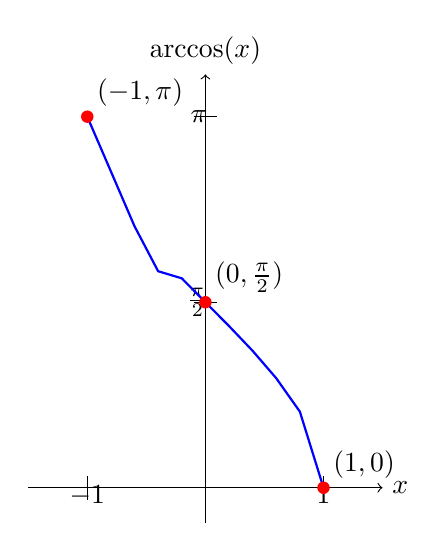
\begin{tikzpicture}[scale=1.5]
  % Ejes
  \draw[->] (-1.5,0) -- (1.5,0) node[right] {$x$};
  \draw[->] (0,-0.3) -- (0,3.5) node[above] {$\arccos(x)$};
  
  % Etiquetas de los ejes
  \draw (-1,-0.1) -- (-1,0.1) node[below] {$-1$};
  \draw (1,-0.1) -- (1,0.1) node[below] {$1$};
  \draw (-0.1,{3.14159}) -- (0.1,{3.14159}) node[left] {$\pi$};
  \draw (-0.1,{1.5708}) -- (0.1,{1.5708}) node[left] {$\frac{\pi}{2}$};
  
  % Gráfica del arcocoseno (aproximación manual con coordenadas)
  \draw[blue, thick] (-1,3.14159) 
    -- (-0.8,2.678) -- (-0.6,2.214) -- (-0.4,1.833) -- (-0.2,1.773)
    -- (0,1.5708) -- (0.2,1.369) -- (0.4,1.159) -- (0.6,0.927) 
    -- (0.8,0.644) -- (1,0);
  
  % Puntos importantes
  \fill[red] (-1,{3.14159}) circle (1.5pt);
  \fill[red] (0,{1.5708}) circle (1.5pt);
  \fill[red] (1,0) circle (1.5pt);
  
  % Etiquetas de puntos
  \node[above right] at (-1,{3.14159}) {$(-1,\pi)$};
  \node[above right] at (0,{1.5708}) {$(0,\frac{\pi}{2})$};
  \node[above right] at (1,0) {$(1,0)$};
\end{tikzpicture}
\end{center}

\begin{center}
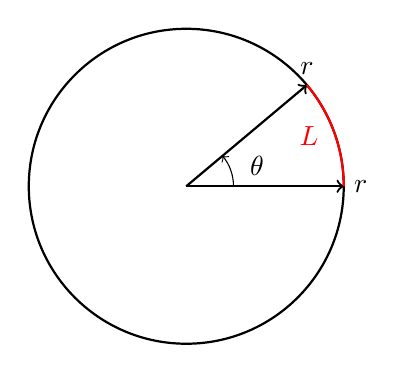
\begin{tikzpicture}[scale=2]
  % Circunferencia
  \draw[thick] (0,0) circle(1);
  % Radio inicial
  \draw[thick,->] (0,0) -- (1,0) node[anchor=west]{$r$};
  % Radio final
  \draw[thick,->] (0,0) -- ({cos(40)},{sin(40)}) node[anchor=south]{$r$};
  % Arco
  \draw[red,thick] (1,0) arc (0:40:1);
  % Ángulo
  \draw[->] (0.3,0) arc (0:40:0.3);
  \node at (0.45,0.13) {$\theta$};
  % Etiqueta del arco
  \node[red] at (0.78,0.32) {$L$};
\end{tikzpicture}
\end{center}

\newpage

% Sección 2 - Fondo blanco
\pagecolor{white}
% Sección: Identidad del coseno de la suma
\section{Identidad del coseno de la suma}\label{sec:identidad}
La identidad trigonométrica para el coseno de la suma de dos ángulos es:
\begin{equation}\label{eq:coseno_suma}
\cos(a + b) = \cos a \cos b - \sin a \sin b
\end{equation}

\newpage

% Sección 3 - Fondo carne
\pagecolor{carne}
\input{03_demostracion_geometrica.tex}
\newpage

% Sección 4 - Fondo blanco
\pagecolor{white}
% Sección: Deducción de la matriz de rotación
\section{Deducción de la matriz de rotación}\label{sec:rotacion}
La matriz de rotación por un ángulo $\theta$ en el plano se deduce así:

Si rotamos el punto $(x, y)$ por un ángulo $\theta$ respecto al origen, las nuevas coordenadas $(x', y')$ son:
\begin{align*}
x' &= x \cos \theta - y \sin \theta \\
y' &= x \sin \theta + y \cos \theta
\end{align*}
Esto se puede escribir en forma matricial:
\begin{equation*}
\begin{pmatrix}
x' \\
y'
\end{pmatrix} =
\begin{pmatrix}
\cos \theta & -\sin \theta \\
\sin \theta & \cos \theta
\end{pmatrix}
\begin{pmatrix}
x \\
y
\end{pmatrix}
\end{equation*}
Por lo tanto, la matriz de rotación es:
\begin{equation*}
R(\theta) = \begin{pmatrix}
\cos \theta & -\sin \theta \\
\sin \theta & \cos \theta
\end{pmatrix}
\end{equation*}

\subsection{Justificación mediante el Teorema de Pitágoras}

La deducción de la matriz de rotación está fundamentada en el teorema de Pitágoras y las definiciones trigonométricas. Consideremos un punto $P(x, y)$ que se encuentra a una distancia $r$ del origen, donde:

\begin{equation*}
r = \sqrt{x^2 + y^2}
\end{equation*}

Si el punto $P$ forma un ángulo $\alpha$ con el eje $x$ positivo, entonces por definición trigonométrica:
\begin{align*}
x &= r \cos \alpha \\
y &= r \sin \alpha
\end{align*}

Al rotar este punto por un ángulo $\theta$, el nuevo ángulo con respecto al eje $x$ será $(\alpha + \theta)$. Las nuevas coordenadas del punto rotado $P'(x', y')$ serán:
\begin{align*}
x' &= r \cos(\alpha + \theta) \\
y' &= r \sin(\alpha + \theta)
\end{align*}

Aplicando las identidades trigonométricas para la suma de ángulos:
\begin{align*}
x' &= r[\cos \alpha \cos \theta - \sin \alpha \sin \theta] \\
y' &= r[\sin \alpha \cos \theta + \cos \alpha \sin \theta]
\end{align*}

Sustituyendo $x = r \cos \alpha$ y $y = r \sin \alpha$:
\begin{align*}
x' &= x \cos \theta - y \sin \theta \\
y' &= x \sin \theta + y \cos \theta
\end{align*}

\textbf{Verificación con el Teorema de Pitágoras:}

Una propiedad fundamental de las rotaciones es que preservan las distancias. Esto significa que:
\begin{equation*}
|P'| = |P| \Rightarrow \sqrt{(x')^2 + (y')^2} = \sqrt{x^2 + y^2}
\end{equation*}

Verificando:
\begin{align*}
(x')^2 + (y')^2 &= (x \cos \theta - y \sin \theta)^2 + (x \sin \theta + y \cos \theta)^2 \\
&= x^2 \cos^2 \theta - 2xy \cos \theta \sin \theta + y^2 \sin^2 \theta \\
&\quad + x^2 \sin^2 \theta + 2xy \sin \theta \cos \theta + y^2 \cos^2 \theta \\
&= x^2(\cos^2 \theta + \sin^2 \theta) + y^2(\sin^2 \theta + \cos^2 \theta) \\
&= x^2 + y^2
\end{align*}

donde hemos usado la identidad pitagórica fundamental $\cos^2 \theta + \sin^2 \theta = 1$.

Esta verificación confirma que la matriz de rotación preserva la magnitud de los vectores, validando así nuestra deducción mediante el teorema de Pitágoras.

\newpage

% Sección 5 - Fondo carne
\pagecolor{carne}
\input{05_demostracion_formula_coseno.tex}
\newpage

% Sección 6 - Fondo blanco
\pagecolor{white}
% Sección: Representación de los números complejos como matrices 2x2
\section{Representación de los números complejos como matrices 2x2}\label{sec:complejos}
Un número complejo $z = a + bi$ puede representarse como la matriz:
\begin{equation*}
M(z) = \begin{pmatrix}
a & -b \\
b & a
\end{pmatrix}
\end{equation*}

Esta matriz actúa sobre vectores en $\mathbb{R}^2$ de la misma forma que la multiplicación por el número complejo $z$.

Por ejemplo, el número complejo $i$ se representa como:
\begin{equation*}
M(i) = \begin{pmatrix}
0 & -1 \\
1 & 0
\end{pmatrix}
\end{equation*}

Esta matriz corresponde a una rotación de $90^\circ$ en el plano.

La multiplicación de matrices de este tipo corresponde a la multiplicación de números complejos.

\newpage

% Sección 7 - Fondo carne
\pagecolor{carne}
% Sección: Ejemplo de rotación de 2\pi/5
\section{Ejemplo: Rotación de $\frac{2\pi}{5}$ como matriz 2x2}\label{sec:ejemplo}
La matriz de rotación por un ángulo $\theta$ en el plano es:
\begin{equation*}
R(\theta) = \begin{pmatrix}
\cos \theta & -\sin \theta \\
\sin \theta & \cos \theta
\end{pmatrix}
\end{equation*}

Para $\theta = \frac{2\pi}{5}$:
\begin{equation*}
R\left(\frac{2\pi}{5}\right) = \begin{pmatrix}
\cos\left(\frac{2\pi}{5}\right) & -\sin\left(\frac{2\pi}{5}\right) \\
\sin\left(\frac{2\pi}{5}\right) & \cos\left(\frac{2\pi}{5}\right)
\end{pmatrix}
\end{equation*}

Aproximando los valores:
\begin{equation*}
\cos\left(\frac{2\pi}{5}\right) \approx 0.3090, \quad \sin\left(\frac{2\pi}{5}\right) \approx 0.9511
\end{equation*}

Además, $\cos\left(\frac{2\pi}{5}\right)$ se puede expresar en términos del número áureo $\varphi$:
\begin{equation*}
\varphi = \frac{1 + \sqrt{5}}{2}
\end{equation*}
\begin{equation*}
\cos\left(\frac{2\pi}{5}\right) = \frac{\varphi - 1}{2}
\end{equation*}

Por lo tanto, la matriz de rotación puede escribirse como:
\begin{equation*}
R\left(\frac{2\pi}{5}\right) = \begin{pmatrix}
\frac{\varphi - 1}{2} & -0.9511 \\
0.9511 & \frac{\varphi - 1}{2}
\end{pmatrix}
\end{equation*}

Esta matriz realiza una rotación de $\frac{2\pi}{5}$ radianes (72 grados) en el plano.

\newpage

% Sección 8 - Fondo blanco
\pagecolor{white}
\input{08_demostracion_coseno_aureo.tex}
\newpage

% Sección 9 - Fondo carne
\pagecolor{carne}
\section{Demostración alternativa de la ecuación para cos(2π/5)}\label{sec:demostracion_alternativa}

Una segunda razón por la cual $\cos\left(\frac{2\pi}{5}\right)$ satisface la ecuación $4x^2 + 2x - 1 = 0$ se basa en las propiedades del pentágono regular y la teoría de números complejos.

\subsection{Enfoque mediante las raíces quintas de la unidad}

Las raíces quintas de la unidad son las soluciones de $z^5 = 1$, dadas por:
\[
z_k = e^{2\pi i k/5} = \cos\left(\frac{2\pi k}{5}\right) + i\sin\left(\frac{2\pi k}{5}\right)
\]
para $k = 0, 1, 2, 3, 4$.

La suma de todas las raíces quintas de la unidad es cero:
\[
\sum_{k=0}^{4} z_k = 1 + z_1 + z_2 + z_3 + z_4 = 0
\]

Por lo tanto: $z_1 + z_2 + z_3 + z_4 = -1$

\subsection{Uso de la simetría}

Observemos que:
\begin{align}
z_1 &= e^{2\pi i/5} = \cos\left(\frac{2\pi}{5}\right) + i\sin\left(\frac{2\pi}{5}\right) \\
z_4 &= e^{8\pi i/5} = \cos\left(\frac{8\pi}{5}\right) + i\sin\left(\frac{8\pi}{5}\right)
\end{align}

Como $\frac{8\pi}{5} = 2\pi - \frac{2\pi}{5}$, tenemos:
\[
z_4 = \cos\left(\frac{2\pi}{5}\right) - i\sin\left(\frac{2\pi}{5}\right) = \overline{z_1}
\]

Similarmente, $z_2 = \overline{z_3}$.

\subsection{Derivación de la ecuación cuadrática}

Sean $\alpha = z_1 + z_4 = 2\cos\left(\frac{2\pi}{5}\right)$ y $\beta = z_2 + z_3 = 2\cos\left(\frac{4\pi}{5}\right)$.

De la suma de raíces: $\alpha + \beta = -1$

Para el producto $\alpha \beta$:
\begin{align}
\alpha \beta &= (z_1 + z_4)(z_2 + z_3) \\
&= z_1 z_2 + z_1 z_3 + z_4 z_2 + z_4 z_3 \\
&= z_3 + z_4 + z_1 + z_2 = -1
\end{align}

Por lo tanto, $\alpha$ y $\beta$ son raíces de la ecuación cuadrática:
\[
t^2 + t - 1 = 0
\]

Como $\alpha = 2\cos\left(\frac{2\pi}{5}\right)$, si hacemos $x = \cos\left(\frac{2\pi}{5}\right)$, entonces $2x$ satisface:
\[
(2x)^2 + (2x) - 1 = 0
\]

Simplificando:
\[
4x^2 + 2x - 1 = 0
\]

Esta es otra demostración de por qué $\cos\left(\frac{2\pi}{5}\right)$ satisface exactamente esta ecuación cuadrática.

\newpage

% Sección 10 - Fondo blanco
\pagecolor{white}
\section{Polinomio de Chebyshev y relacion con Fibonacci}\label{sec:chebfib}

\subsection{Puntos por hacer}
\begin{itemize}
  \item[$\square$] Agregar ejemplos adicionales de polinomios de Chebyshev
  \item[$\square$] Relacionar con otras funciones trigonométricas
\end{itemize}

Los polinomios de Chebyshev $T_n(x)$ son una familia de polinomios definidos por:
\begin{equation}\label{eq:def_chebyshev}
T_n(x) = \cos(n \arccos x)
\end{equation}

Son útiles porque relacionan los cosenos de múltiplos de un ángulo con potencias de $x = \cos \theta$. Por ejemplo, para $n=5$:
\begin{equation}\label{eq:T5_chebyshev}
T_5(x) = 16x^5 - 20x^3 + 5x
\end{equation}

La identidad $\cos(5\theta) = T_5(\cos \theta)$ permite obtener ecuaciones polinómicas para los cosenos de múltiplos de un ángulo, como se usó en \eqref{eq:chebyshev_identity}.

\subsection{Demostracion de los polinomios de Chebyshev}

\subsection{Puntos por hacer}
\begin{itemize}
  \item[$\square$] Incluir demostración gráfica
  \item[$\square$] Agregar ejercicios de recurrencia
\end{itemize}

Los polinomios de Chebyshev $T_n(x)$ se definen recursivamente:
\begin{align}
T_0(x) &= 1 \label{eq:T0_chebyshev}\\
T_1(x) &= x \label{eq:T1_chebyshev}\\
T_{n+1}(x) &= 2x T_n(x) - T_{n-1}(x) \label{eq:recurrencia_chebyshev}
\end{align}

Por ejemplo:
\begin{align*}
T_2(x) &= 2x T_1(x) - T_0(x) = 2x^2 - 1 \\
T_3(x) &= 2x T_2(x) - T_1(x) = 4x^3 - 3x \\
T_4(x) &= 2x T_3(x) - T_2(x) = 8x^4 - 8x^2 + 1 \\
T_5(x) &= 2x T_4(x) - T_3(x) = 16x^5 - 20x^3 + 5x
\end{align*}

Estos polinomios cumplen la identidad:
\begin{equation*}
T_n(x) = \cos(n \arccos x)
\end{equation*}

Por eso, si $x = \cos \theta$, entonces $T_5(x) = \cos(5\theta)$, lo que permite obtener ecuaciones polinómicas para los cosenos de múltiplos de un ángulo.

\subsection{Relacion entre Chebyshev y Fibonacci}

\subsection{Puntos por hacer}
\begin{itemize}
  \item[$\square$] Profundizar en la relación con la sucesión de Fibonacci
  \item[$\square$] Ejemplos numéricos
\end{itemize}

Existe una relación entre los polinomios de Chebyshev y la sucesión de Fibonacci. Si evaluamos el polinomio de Chebyshev de segundo tipo $U_n(x)$ en $x = \frac{1}{2}$, obtenemos:
\begin{equation*}
U_n\left(\frac{1}{2}\right) = F_{n+1}
\end{equation*}
donde $F_{n+1}$ es el número de Fibonacci de orden $n+1$.

Además, para el polinomio de Chebyshev de primer tipo $T_n(x)$, existe la relación:
\begin{equation*}
T_n\left(\frac{1}{2}\right) = \frac{1}{2} F_n
\end{equation*}

Esto se debe a que ambos cumplen relaciones de recurrencia similares y están conectados a través de funciones trigonométricas e hiperbólicas.

Por ejemplo:
\begin{align*}
T_5\left(\frac{1}{2}\right) &= 16\left(\frac{1}{2}\right)^5 - 20\left(\frac{1}{2}\right)^3 + 5\left(\frac{1}{2}\right) \\
&= 0.5
\end{align*}
que corresponde a $\frac{1}{2} F_5$ ya que $F_5 = 5$.

\subsection{Polinomios de Chebyshev y su relacion trigonometrica}

\subsection{Puntos por hacer}
\begin{itemize}
  \item[$\square$] Agregar ejemplos con valores específicos de theta
  \item[$\square$] Incluir aplicaciones en física y matemáticas
\end{itemize}

Sea $P_0(x) = 1$, $P_1(x) = x$ y para $n > 1$:
\[
    P_{n+1}(x) = x P_n(x) - P_{n-1}(x)
\]
Estos son los polinomios de Chebyshev de primer tipo, definidos por recurrencia.

Ahora, demostraremos que:
\[
    P_n(2 \cos \theta) = \frac{\sin(n+1)\theta}{\sin \theta}
\]

\textbf{Demostración:}

Consideremos la recurrencia para $P_n(x)$ y tomemos $x = 2 \cos \theta$.

Definimos $S_n = \sin(n\theta)$.

Sabemos que:
\[
    S_{n+1} = 2 \cos \theta S_n - S_{n-1}
\]

Esto es la misma recurrencia que para $P_n(x)$ con $x = 2 \cos \theta$.

\subsection{Puntos por hacer}
\begin{itemize}
  \item[$\square$] Verificar casos base
  \item[$\square$] Completar demostración por inducción
  \item[$\square$] Agregar ejemplos numéricos
\end{itemize}

Por inducción:
\begin{itemize}
\item Para $n=0$: $P_0(2\cos\theta) = 1 = \frac{\sin(\theta)}{\sin\theta}$
\item Para $n=1$: $P_1(2\cos\theta) = 2\cos\theta = \frac{\sin(2\theta)}{\sin\theta}$
\end{itemize}

Supongamos que $P_n(2\cos\theta) = \frac{\sin((n+1)\theta)}{\sin\theta}$ y $P_{n-1}(2\cos\theta) = \frac{\sin(n\theta)}{\sin\theta}$.

Entonces:
\begin{align}
P_{n+1}(2\cos\theta) &= 2\cos\theta P_n(2\cos\theta) - P_{n-1}(2\cos\theta) \\
&= 2\cos\theta \frac{\sin((n+1)\theta)}{\sin\theta} - \frac{\sin(n\theta)}{\sin\theta} \\
&= \frac{2\cos\theta \sin((n+1)\theta) - \sin(n\theta)}{\sin\theta}
\end{align}

Usando la identidad trigonométrica:
\[
    2\cos\theta \sin((n+1)\theta) = \sin((n+2)\theta) + \sin(n\theta)
\]

Por lo tanto:
\[
    P_{n+1}(2\cos\theta) = \frac{\sin((n+2)\theta) + \sin(n\theta) - \sin(n\theta)}{\sin\theta} = \frac{\sin((n+2)\theta)}{\sin\theta}
\]

Esto completa la inducción y la demostración.

\subsection{Puntos por hacer}
\begin{itemize}
  \item[$\square$] Agregar conexión con Fibonacci
  \item[$\square$] Incluir gráficas comparativas
  \item[$\square$] Verificar con ejemplos específicos
\end{itemize}

\newpage

% Conclusión - Fondo blanco
\pagecolor{white}
\section{Conclusión}\label{sec:conclusion}
La fórmula se demuestra usando la composición de rotaciones en el plano, y se verifica algebraicamente con matrices de rotación.

\end{document}
